\newpage

\section{평가}
\label{sec:evaluation}
\begin{figure}[h!]
  \begin{center}
    \includegraphics[scale=1.2]{fig/xeon}
  \end{center}
  \caption{실험 환경.}
  \label{fig:xeon}
\end{figure}


\begin{figure}[tb]
  \begin{center}
    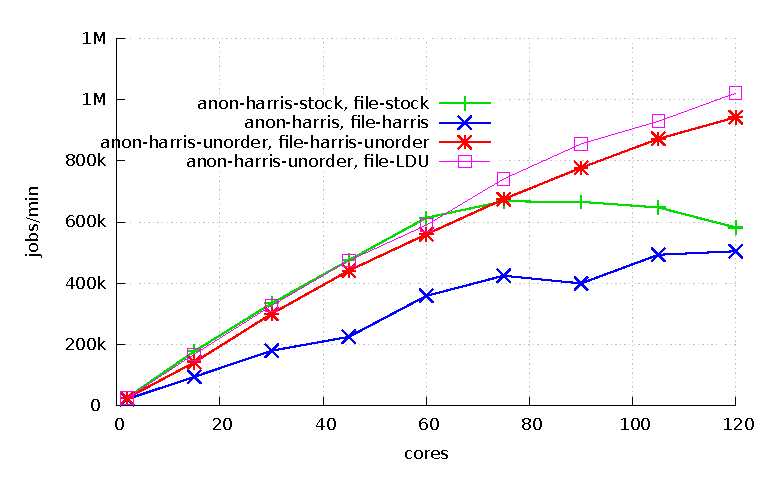
\includegraphics[scale=0.8]{graph/aim7.eps}
  \end{center}
  \caption{AIM7-multiuser 확장성.}
  \label{fig:aim7}
\end{figure}


\begin{figure*}[tb]
    \centering
    \begin{subfigure}[b]{1\textwidth}
  \begin{center}
        \includegraphics[scale=0.8]{graph/aim7_cpuutils.eps}
  \end{center}
    \end{subfigure}%
    \centering
    \caption{120코어에서 AIM7 CPU 사용량.}
    \label{fig:utilization_aim7}
    
\end{figure*}


\begin{figure*}[tb]
    \centering
    \begin{subfigure}[b]{1\textwidth}
  \begin{center}
        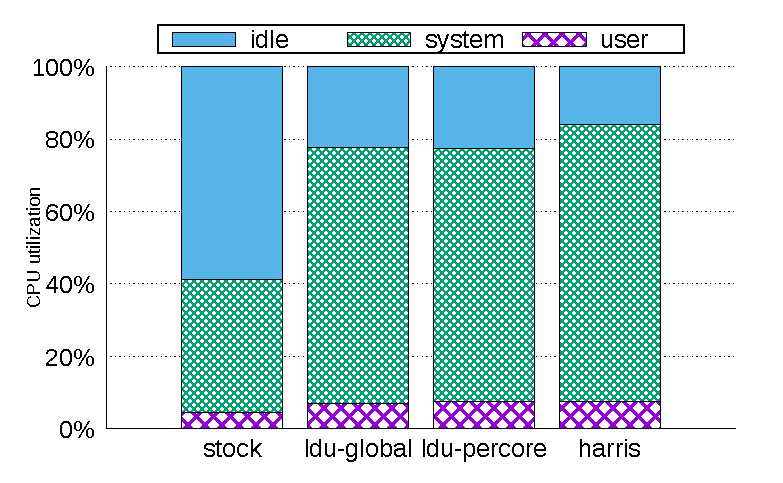
\includegraphics[scale=0.8]{graph/exim_cpuutils.eps}
  \end{center}
    \end{subfigure}
    \centering
    \caption{120코어에서 EXIM CPU 사용량. }
    \label{fig:utilization_exim}
    
\end{figure*}



\begin{figure*}[tb]
    \centering
    \begin{subfigure}[b]{1\textwidth}
  \begin{center}
        \includegraphics[scale=0.8]{graph/lmbench_cpuutils.eps}
  \end{center}
    \end{subfigure}
        \centering
    \caption{120코어에서 Lmbench CPU 사용량.}
    \label{fig:utilization_lmbench}
    
\end{figure*}



\subsection{실험 환경}


%$$$$$$$$$$$$$$$$$$$$$$$$$$$$$$$$$$$$$$$$$$$$$$$$$$$$$$$$$$$$$$$$$$$$$$$$$$$$$$$$
%Paragraph 1: 무엇을 평가 했는지에 대한 설명 
%$$$$$$$$$$$$$$$$$$$$$$$$$$$$$$$$$$$$$$$$$$$$$$$$$$$$$$$$$$$$$$$$$$$$$$$$$$$$$$$$

%For the purpose of performance evaluation of the proposed 
%\LDU technique, we performed experiments using a Linux kernel
%where \LDU technique is implemented compared to a lock-free list
%version of Linux proposed by Harris~\cite{Harris2001Lockfree}.
우리가 제안한 LDU 기법에 대해서 평가를 하기 위해, 우리는 리눅스 커널에 LDU를 적용하여 비교하였다.
비교 대상으로는 수정하지 않은 리눅스 커널과 Harris의 Lock-free 리스트~\cite{Harris2001Lockfree}를
 구현하여 비교 실험을 하였다.
%The reason why we used Harris algorithm for our comparison 
%purposes is that the algorithm is considered as the representative
%concurrent non-blocking algorithm.
Harris 알고리즘을 사용한 이유는 논블락킹 알고리즘 중에서 대표하는 알고리즘이기 때문이다. 
%The basic algorithms of Harris linked list are from
% sysnchrobench~\cite{Gramoli2015Synchrobench}
%and ASCYLIB~\cite{David2015ASYNCHRONIZED}, and we slightly converted the
%Harris linked list to be adopted in Linux kernels.
Harris의 링크드 리스트의 기본적인 알고리즘은 sysnchrobench~\cite{Gramoli2015Synchrobench}과
ASCYLIB~\cite{David2015ASYNCHRONIZED}에서 구현된 내용을 사용했으며, 우리는 이러한 Harris 링크드 
리스트를  리눅스 커널에 적용하였다. 

%$$$$$$$$$$$$$$$$$$$$$$$$$$$$$$$$$$$$$$$$$$$$$$$$$$$$$$$$$$$$$$$$$$$$$$$$$$$$$$$$
%Paragraph 3: 운영체제 및 커널 버전 설명
%$$$$$$$$$$$$$$$$$$$$$$$$$$$$$$$$$$$$$$$$$$$$$$$$$$$$$$$$$$$$$$$$$$$$$$$$$$$$$$$$
%The hardware specification we used for our experiments
%are a 120 core machine with 8-socket, Intel
%E7-8870 chips(15 cores per socket) equipped with 792 GB DDR3 DRAM.
실험을 위해 우리가 사용한 하드웨어 명세서는 8소켓으로 구성된 120코어 시스템을 사용했으며,
각각의 코어는 인텔 E7-8870 chips(15 cores per socket)을 사용했다.
메모리는 792기가 바이트 DDR3 DRAM을 사용하였다.
그림~\ref{fig:xeon}은 우리가 사용한 시스템을 보여준다.


%$$$$$$$$$$$$$$$$$$$$$$$$$$$$$$$$$$$$$$$$$$$$$$$$$$$$$$$$$$$$$$$$$$$$$$$$$$$$$$$$
%Paragraph 2-1: Harris Lock free list 구현 내용에 대한 설명 
%$$$$$$$$$$$$$$$$$$$$$$$$$$$$$$$$$$$$$$$$$$$$$$$$$$$$$$$$$$$$$$$$$$$$$$$$$$$$$$$$
%To compare our the \LDU implementation to a concurrent non-blocking
%algorithm, we additionally implemented the
%Harris linked list~\cite{Harris2001Lockfree} to Linux kernel.
%The Harris linked list refers from sysnchrobench~\cite{Gramoli2015Synchrobench}
%and ASCYLIB~\cite{David2015ASYNCHRONIZED}, and we slightly converted the
%Harris linked list to the Linux kernel style.
%Then, we replaced the two interval tree to the Harris linked list.
%In addition, since the Harris linked list in the synchrobench and the ASCYLIB leaks memory,
%we implemented a garbage collector for Linux kernel using the Linux work
%queues and non-blocking linked list.

%$$$$$$$$$$$$$$$$$$$$$$$$$$$$$$$$$$$$$$$$$$$$$$$$$$$$$$$$$$$$$$$$$$$$$$$$$$$$$$$$
%Paragraph 1: 벤치 마크 대한 설명
%$$$$$$$$$$$$$$$$$$$$$$$$$$$$$$$$$$$$$$$$$$$$$$$$$$$$$$$$$$$$$$$$$$$$$$$$$$$$$$$$
%We selected benchmark programs with fork-intensive applications since the
%fork-intensive update-heavy data structure accesses could maximally benefit
%from the proposed technique.
우리는 리눅스 fork에 집약적인 응용프로그램과 업데이트 비율이 많은 자료구조가 우리가 
제안한 방법에 효율적이기 때문에 fork에 집약적인 벤치마크를 선택하였다. 
%The benchmark programs are AIM7, a Linux
%scalability benchmark, Exim, an email server in MOSBENCH, and Lmbench, a micro
% benchmark.
이러한 벤치마크 프로그램들은 리눅스의 확장성 벤치마크인 AIM7, 그리고 MOSBENCH에서
 이메일 서버 벤치마크인 Exim 그리고 마이크로 벤치마크인 Lmbench 이다.
%The workloads exhibit the high lock contentions because of the two reverse
% mappings.
이러한 워크로드 들은 두가지 역 매핑 때문에 높은 락 경합을 보여준다. 
%Moreover, the AIM7 benchmark is widely used in the Linux community not only for
%testing Linux kernel but also for improving the scalability. 
더욱이, AIM7 벤치마크는 리눅스 커뮤니티에서 리눅스 커널에 대한 테스팅 뿐만 아니라 확장성을 향상 
시키기 위해 많이 사용되는 벤치마크이다.
%The Exim is a real world application, but it has scalability bottlenecks caused
%by the Linux fork.
Exim은 실제 사용되고 있는 응용프로그램이다. 하지만 이것 역시 리눅스 fork 때문에 
성능에 병목 문제가 생긴다.
%Finally, in order to only focus on the fork performance and scalability, we
%selected the Lmbench.
마지막으로 우리는 fork에 대한 성능과 확장성에 대해서 보기위해 우리는 Lmbench를 
선택하였다. 

%$$$$$$$$$$$$$$$$$$$$$$$$$$$$$$$$$$$$$$$$$$$$$$$$$$$$$$$$$$$$$$$$$$$$$$$$$$$$$$$$
%Paragraph 2: 비교 대상에 대한 설명
%$$$$$$$$$$$$$$$$$$$$$$$$$$$$$$$$$$$$$$$$$$$$$$$$$$$$$$$$$$$$$$$$$$$$$$$$$$$$$$$$
%We used four different experiment settings. 
우리는 비교를 위해 4가지 다른 설정으로 실험하였다. 
%First, we used the stock Linux as the baseline reference. 
첫째로, 우리는 기본 점수를 보기 위해, 수정없는 리눅스 커널(stock linux)을 사용하였다.
%Second, we used the \LDU version of Linux kernel that used global queue.
둘째로, 우리는 전역 큐 버전의 LDU를 사용해서 실험하였다.  
%Next, we used the per-core queue version of the \LDU.
다음으로, 우리는 퍼코어 버전의 LDU를 사용하여 실험하였다. 
%Finally, we used Harris lock-free list version of Linux kernel as we
%mentioned earlier.
마지막으로 우리는 앞에서 설명한 Harris의 lock-free 링크드 리스트 버전의 리눅스 커널을 대상으로 
실험하였다.  
%Unfortunately, direct comparison experiments between the \LDU and the OpLog was
% not possible for a few implementation-related issues (e.g., we could not
 % obtain the detailed implementation of the OpLog).
안타깝게도, LDU와 OpLog를 몇몇의 구현 관련 이슈(우리는 OpLog의 자세한 구현을 얻지 못하였다.)로
 인해 바로 비교하지 못하였다.

\subsection{AIM7}

%$$$$$$$$$$$$$$$$$$$$$$$$$$$$$$$$$$$$$$$$$$$$$$$$$$$$$$$$$$$$$$$$$$$$$$$$$$$$$$$$
%Paragraph 1: AIM7 실험 결과
%$$$$$$$$$$$$$$$$$$$$$$$$$$$$$$$$$$$$$$$$$$$$$$$$$$$$$$$$$$$$$$$$$$$$$$$$$$$$$$$$


%$$$$$$$$$$$$$$$$$$$$$$$$$$$$$$$$$$$$$$$$$$$$$$$$$$$$$$$$$$$$$$$$$$$$$$$$$$$$$$$$
%Paragraph 1: 워크로드에 대한 설명
%$$$$$$$$$$$$$$$$$$$$$$$$$$$$$$$$$$$$$$$$$$$$$$$$$$$$$$$$$$$$$$$$$$$$$$$$$$$$$$$$
%We used AIM7-multiuser, which is one of fork-intensive workload in AIM7.
우리는 AIm7-multiuser를 사용하였다. 이것은 AIM7의 워크로드 중 리눅스 fork에 집중된 벤치마크이다. 
%The multiuser workload simultaneously creates many processes with various
%operations(see section~\ref{sec:bg}), and we used the temp filesystem to
% minimize the file system bottleneck.
이러한 multiuser 워크로드는 동시에 많은 프로세스를 생성 한 후 다양한
 일을 수행한다(see section~\ref{sec:bg}).
 또한, 우리는 파일 시스템에 대한 병목현상을 줄이기 위해 리눅스 temp 파일 시스템을 사용하였다. 
%We increased a number of users in proportion to number of cores.
우리는 코어 수에 비례하여 user들을 증가하였다. 
 
%$$$$$$$$$$$$$$$$$$$$$$$$$$$$$$$$$$$$$$$$$$$$$$$$$$$$$$$$$$$$$$$$$$$$$$$$$$$$$$$$
%Paragraph 2: 실험 결과에 대한 설명
%$$$$$$$$$$$$$$$$$$$$$$$$$$$$$$$$$$$$$$$$$$$$$$$$$$$$$$$$$$$$$$$$$$$$$$$$$$$$$$$$
%The results for AIM7-multiuser are shown in Figure~\ref{fig:aim7}.
AIM7-multiuser에 대한 실험 결과는 그림 ~\ref{fig:aim7}과 같다.
%Up to 75 core, the stock Linux scales linearly and then serialized updates
%become bottlenecks.
75코어 전 까지는 수정 안한 리눅스는 확장성이 일정하나 그 이후에는 직렬화된 업데이트들 때문에
병목현상이 생긴다. 
%However, up to 120 core, the Harris and our \LDU scale well because
%these workloads can concurrently execute update operations without the
%reader-writer semaphores(\code{anon\_vma->rwsem},
% \code{mapping->i\_mmap\_rwsem}).
하지만, 120코어까지 Harris 링크드 리스트와 우리의 LDU는 확장성이 있다. 
그 이유는 워크로드들이 업데이트 명령어와 읽기-쓰기 세마포어(\code{anon\_vma->rwsem},
\code{mapping->i\_mmap\_rwsem}) 없이 동시적으로 실행되기 때문이다.
%The per-core queue version of the \LDU shows the best performance and
%scalability outperforming stock Linux by 1.5x and Harris by
%1.1x.
LDU의 퍼코어 큐버전은 가장 좋은 성능을 보여주고, 확장성도 뛰어나며, 
수정 안 한 리눅스에 비해 1.5배 빠르고 Harris보다 1.1x 빠르다.

%In addition, although the global queue version of the \LDU has the global CAS
% operation, it also has high performance and scalability because the global CAS operations are
%mitigated by two \LDU techniques;it had 2\% performance degradation compared
% with per-core queue version of the \LDU.
게다가, 비록 LDU의 전역 큐버전은 전역 CAS 명령어를 실행하지만, 이 방법 역시 높은 성능과 확장성을 가진다.
그 이유는 LDU의 2가지 기법 때문에 전역 CAS에 대한 접근이 완화되었기 때문이다.
이것은 퍼코어 큐 버전에 비해 2\% 성능 저하가 생긴다. 
%Furthermore, the stock Linux shows the highest idle time(58\%)(see
% figure~\ref{fig:utilization_aim7}) since it waits to acquire semaphore(i.e.,
%\code{anon\_vma->rwsem}, \code{mapping->i\_mmap\_rwsem}).
% Surprisingly, although two \LDU have higher idle time than the Harris version,
%the throughput shows higher than the Harris because of our efficient algorithm.
더욱이, 수정 안 한 리눅스는 가장 높은 유휴(IDLE) 시간(56\%)을 가진다(그림 ~\ref{fig:utilization_aim7}). 
그 이유는 2가지 세마포어(i.e.,
\code{anon\_vma->rwsem}, \code{mapping->i\_mmap\_rwsem}))를 얻기 위해 기다리기 때문이다.
놀랍게도 비록 2가지 LDU가 Harris 커널 버전보다 높은 유휴시간을 가지지만, 처리량은 Harris 방법보다 더 높다.
이것은 바로 우리의 효율적인 알고리즘 때문이다. 

\begin{figure}[tb]
  \begin{center}
    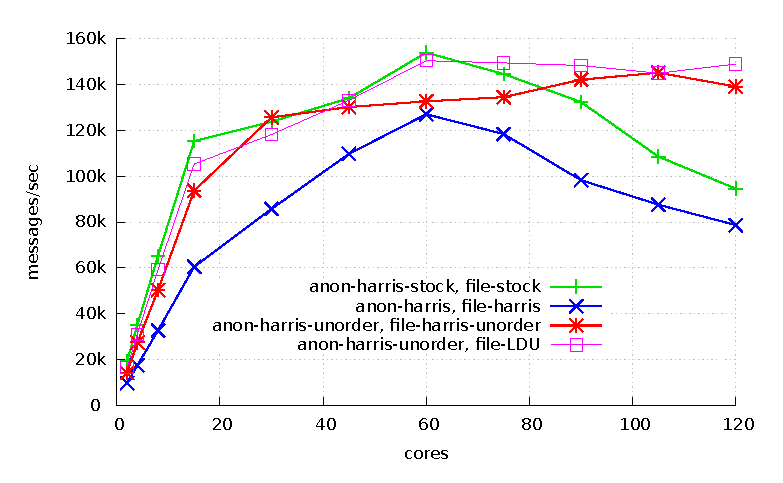
\includegraphics[scale=0.8]{graph/exim.eps}
  \end{center}
  \caption{Exim 확장성.}
  \label{fig:exim}
\end{figure}

\subsection{Exim}
%$$$$$$$$$$$$$$$$$$$$$$$$$$$$$$$$$$$$$$$$$$$$$$$$$$$$$$$$$$$$$$$$$$$$$$$$$$$$$$$$
%Paragraph 1:  EXIM 실험 결과
%$$$$$$$$$$$$$$$$$$$$$$$$$$$$$$$$$$$$$$$$$$$$$$$$$$$$$$$$$$$$$$$$$$$$$$$$$$$$$$$$

\begin{figure}[tb]
  \begin{center}
    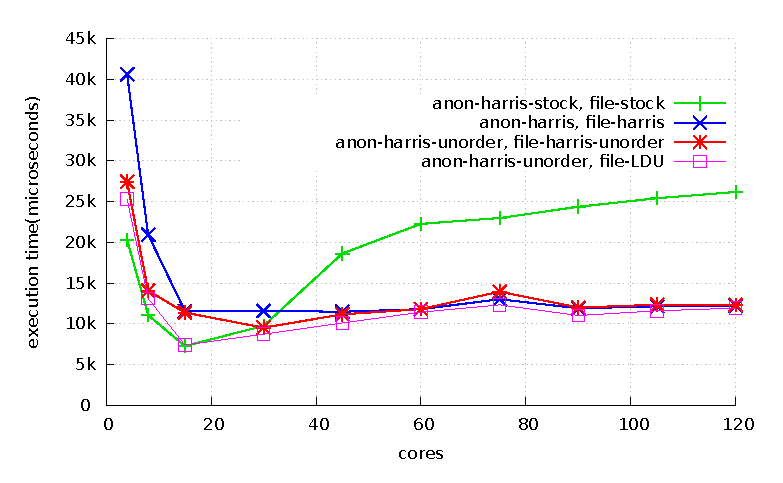
\includegraphics[scale=0.8]{graph/lmbench.eps}
  \end{center}
  \caption{Lmbench의 프로세스 관리 벤치마크에 대한 실행시간.}
  \label{fig:MicroBench}
\end{figure}

%$$$$$$$$$$$$$$$$$$$$$$$$$$$$$$$$$$$$$$$$$$$$$$$$$$$$$$$$$$$$$$$$$$$$$$$$$$$$$$$$
%Paragraph 1: 워크로드에 대한 설명
%$$$$$$$$$$$$$$$$$$$$$$$$$$$$$$$$$$$$$$$$$$$$$$$$$$$$$$$$$$$$$$$$$$$$$$$$$$$$$$$$
%To measure the performance of the Exim, we used the MOSBENCH, a many-core
%scalability benchmark.
Exim의 성능에 대한 확장성을 측정하기 위하여, 우리는 매니코어 확장성 벤치마크 중 하나인
 MOSBENCH를 이용하였다. 
%The Exim email server is designed to scale because the Exim delivers messages
% to mail boxes in parallel using the Linux process;the Exim is a fork-intensive
% workload.
이메일(E-mail) 서버인 Exim의 디자인은 확장성이 있게 설계되었다. 그 이유는 Exim의 메시지(message)
전달자(delivers)는 리눅스의 프로세스를 사용하여 병렬적인 방법을 사용하여 메시지를 메일 박스에 전달한다. 
이러한 Exim은 Fork가 많이 발생하는 워크로드 중 하나이다. 
%Clients ran on the same machine and each client sent to a different user to
%prevent contention on user mail file.
클라이언트는 같은 장치에서 실행되고, 각각의 클라인언트는 메일 파일에 대해서 충돌을 막기 위해
 다른 여러 유저에게 보낸다 
%The Exim was bottlenecked by the
% filesystem~\cite{SilasBoydWickizer2010LinuxScales48} since the message body
% appends to the per-user mail file, so we used the separated tmpfs to reduce
% filesystem bottlenecks.
Exim은 파일 시스템에서 병목이 발생한다~\cite{SilasBoydWickizer2010LinuxScales48}.
그 이유는 메시지의 바디(body)는 각각의 유저 메일 파일에 추가되기 때문이다.
따라서 우리는 파일 시스템의 병목 지점을 제거하기 위해 분활된 tmpfs를 사용하였다. 

%$$$$$$$$$$$$$$$$$$$$$$$$$$$$$$$$$$$$$$$$$$$$$$$$$$$$$$$$$$$$$$$$$$$$$$$$$$$$$$$$
%Paragraph 2:실험 결과에 대한 설명
%$$$$$$$$$$$$$$$$$$$$$$$$$$$$$$$$$$$$$$$$$$$$$$$$$$$$$$$$$$$$$$$$$$$$$$$$$$$$$$$$
%Results shown in figure~\ref{fig:exim} indicate that the Exim scales well up to
%60 core, but the stock Linux performance decreases near 60 core.
그림~\ref{fig:exim}에서 보여주는 Exim의 결과는 수정안한 리눅스 커널의 Exim은
 60코어 까지 확장성이 좋게 동작을 하지만 그 60코어 근처부터 성능이 떨어지는 모습을 볼 수 있다. 
%Both the Harris and the \LDU increase up to 105 core because they can execute
%concurrent updates without the semaphores.
Harris와 우리의 LDU는 105코어까지 성능향상이 보인다. 그 이유는 이 두 방법은 세마포어 때문에 
기다리는 현상이 없이 동시에 업데이트가 명령이 수행할 수 있기 때문이다. 
%The per-core queue version of the \LDU performs better due to the fact that it
% can reduce cache coherence-related overheads outperforming stock Linux by 2.6x and Harris
%by 1.2x.
LDU의 퍼코어 큐 버전은 보다 더 좋은 성능을 가진다.
그 이유는 이것은 캐시 일관성과 관련한 오버헤드를 줄였기 때문이며, 이것은 수정 안한 리눅스보다 2.6배 성능향상을
 가지며 Harris 보다 1.2배의 성능 향상을 한다. 
%Even though we applied the scalable solutions, the Exim shows the limitation
%near 105 core since the Exim process has a relatively large size of virtual
%address mapping that leads to the clearing virtual address mappings overheads
%and many soft page fault during the process destruction which executes more
%slowly with more remote socket memory access.
비록 우리의 확장성이 있는 기술을 적용하였지만, Exim은 105코어부터 성능 확장성에 대해서 문제가 생긴다.
그 이유는 Exim의 프로세스들은 상대적으로 큰 크기의 가상메모리를 사용하기 때문이다.
 이것은 결국 프로세스가 종료될 때 가상메모리에 대한 초기화 오버헤드를 낳으며,
  많은 소프트 페이지 폴트(soft page fault)를 야기 시킨다. 이것은 NUMA 구조와 같은 원격 메모리 접근일 때보다 많은 오버헤드가 발생한다. 
%The Harris has 15\% idle time, whereas per-core queue version of the \LDU
%has 22\% idle time because the \LDU has the efficient algorithm(see
%figure~\ref{fig:utilization_exim}).
Harris 링크드 리스트는 15\%의 유휴 시간을 가진 반면, 퍼코어 큐 버전의 LDU는 22\%의 유휴 시간을 가진다.
그 이유는 LUD의 효율적인 알고르즘 때문이다(그림~\ref{fig:utilization_exim})..

\begin{figure*}[t!]
    \centering
    \begin{subfigure}[b]{1\textwidth}
  \begin{center}
        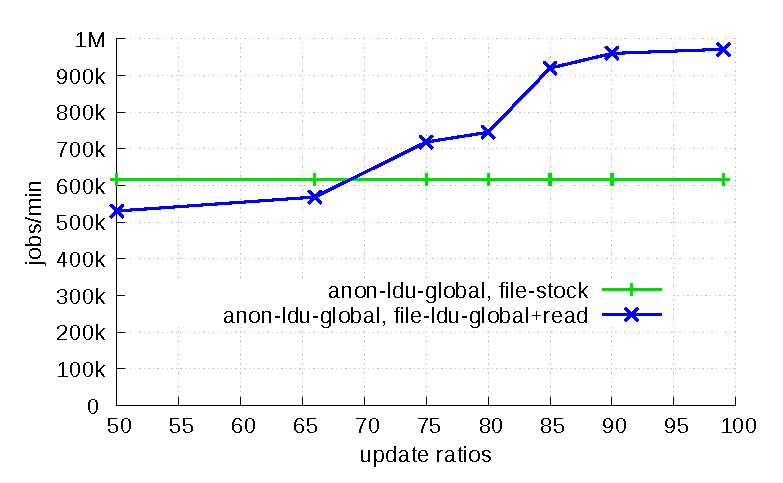
\includegraphics[height=2.5in]{graph/ratio_aim7.eps}
  \end{center}
    \end{subfigure}%
    \caption{업데이트 비율에 따른 AIM7 성능.}
    \label{fig:UpdateRate_aim7}
\end{figure*}

\begin{figure*}[t!]
    \centering
    \begin{subfigure}[b]{1\textwidth}
        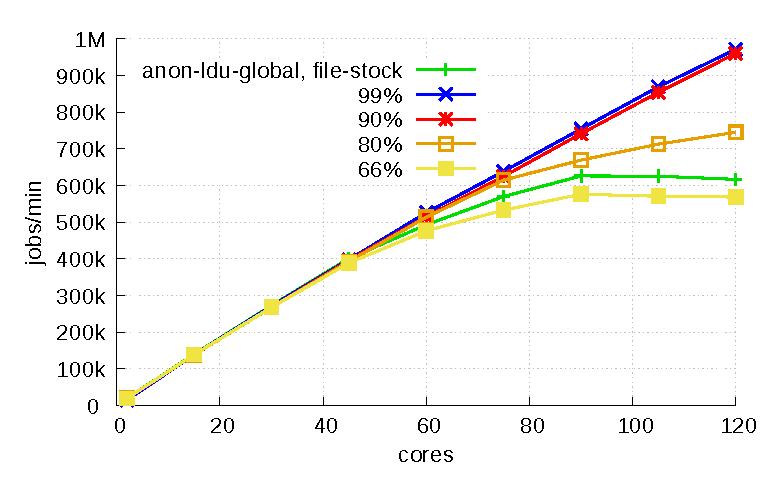
\includegraphics[height=2.5in]{graph/ratio_aim7_core.eps}
    \end{subfigure}%
    \caption{업데이트 비율에 따른 AIM7 확장성.}
    \label{fig:UpdateRate_aim7_2}
\end{figure*}

\begin{figure*}[t!]
    \centering
    \begin{subfigure}[b]{1\textwidth}
  \begin{center}
        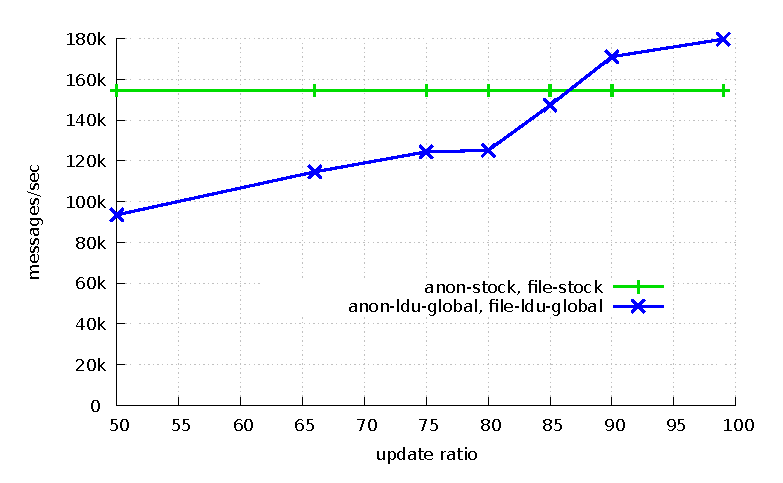
\includegraphics[height=2.5in]{graph/ratio_exim.eps}
  \end{center}
    \end{subfigure}%
    \caption{업데이트 비율에 따른 Exim 성능.}
    \label{fig:UpdateRate_exim}
\end{figure*}

\begin{figure*}[t!]
    \centering
    \begin{subfigure}[b]{1\textwidth}
        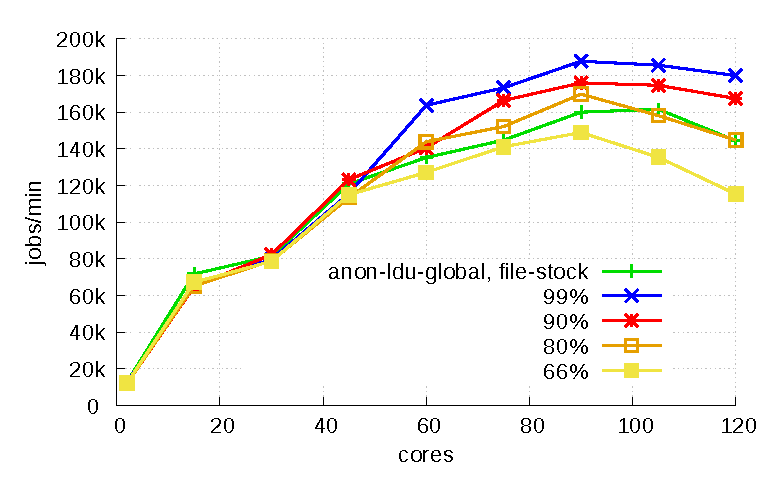
\includegraphics[height=2.5in]{graph/ratio_exim_core.eps}
    \end{subfigure}%
    \caption{업데이트 비율에 따른 Exim 확장성.}
    \label{fig:UpdateRate_exim_2}
\end{figure*}

\begin{figure*}[t!]
    \centering
    \begin{subfigure}[b]{1\textwidth}
  \begin{center}
        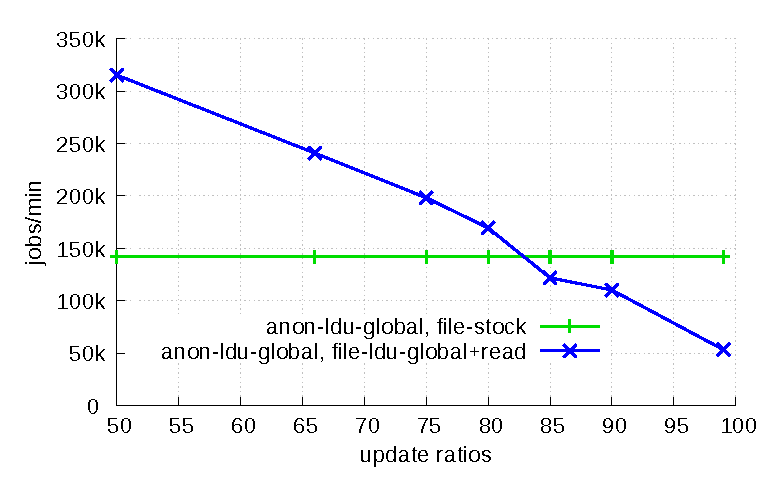
\includegraphics[height=2.5in]{graph/ratio_lmbench.eps}
  \end{center}
    \end{subfigure}%
    \caption{Lmbench performance depending on update ratios.}
    \caption{업데이트 비율에 따른 Lmbench 성능.}
    \label{fig:UpdateRate_lmbench}
\end{figure*}

\begin{figure*}[t!]
    \centering
    \begin{subfigure}[b]{1\textwidth}
        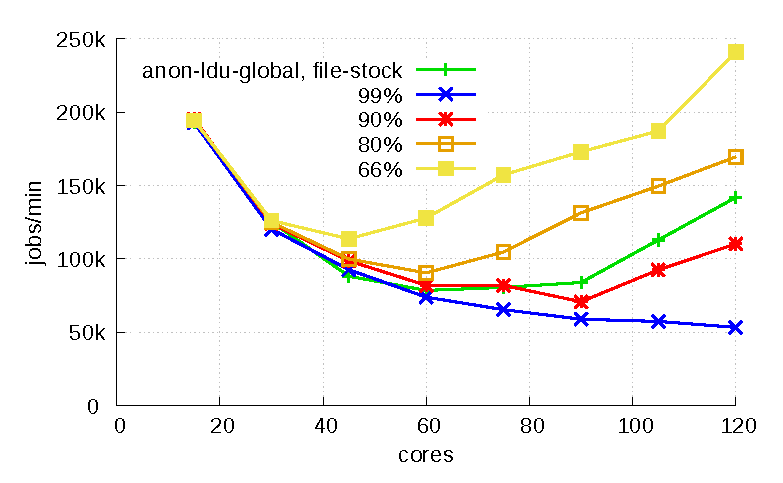
\includegraphics[height=2.5in]{graph/ratio_lmbench_core.eps}
    \end{subfigure}%
    \caption{업데이트 비율에 따른 Lmbench 확장성.}
    \label{fig:UpdateRate_lmbench_2}
\end{figure*}


\subsection{Lmbench}
%$$$$$$$$$$$$$$$$$$$$$$$$$$$$$$$$$$$$$$$$$$$$$$$$$$$$$$$$$$$$$$$$$$$$$$$$$$$$$$$$
%Paragraph 1: %워크로드에 대한 설명
%$$$$$$$$$$$$$$$$$$$$$$$$$$$$$$$$$$$$$$$$$$$$$$$$$$$$$$$$$$$$$$$$$$$$$$$$$$$$$$$$
%The Lmbench has various micro benchmarks including process management
% workloads.
Lmbench는 내부에 프로세스 관리에 대한 워크로드를 포함하여
 다양한 마이크로(micro) 벤치마크를 포함하고 있다. 
%We used the process management workload in the Lmbench.
우리는 이러한 다양한 마이크로 벤치마크 중 프로세스 관리에 대한 워크로드를 사용하였다. 
%This workload is used to measure the basic process primitives such as creating
% a new process, running a program, and context switching.
이러한 워크로드는 기본적인 프로세스 관리에 대한 요소들 예를 들어 프로세스 생성(creating a new process),
 프로그램 시작(running a program) 그리고 문맥교환(context switching) 들을 측정한다.
%We configured process create workload to enable the parallelism option(the
%value was 1000).
그리고 우리는 프로세스 생성에 대한 워크로드를 병렬 옵션(값은 1000)과 함께 설정하여 수행하였다. 

%$$$$$$$$$$$$$$$$$$$$$$$$$$$$$$$$$$$$$$$$$$$$$$$$$$$$$$$$$$$$$$$$$$$$$$$$$$$$$$$$
%Paragraph 2: 실험 결과에 대한 설명
%$$$$$$$$$$$$$$$$$$$$$$$$$$$$$$$$$$$$$$$$$$$$$$$$$$$$$$$$$$$$$$$$$$$$$$$$$$$$$$$$
%The results for the Lmbench are shown in Figure~\ref{fig:MicroBench}, 
%and the results show the execution times.
Lmbench의 결과는 그림~\ref{fig:MicroBench}에서 보여주며, 세로축에 대한 결과는 실행 시간이다.
%Up to 45 core, the stock Linux scales linearly and then the execution time goes
%up to grow.
45코어까지, 수정 안 한 리눅스 커널은 일정한 확장성을 보이며, 그 후 실행시간을 늘어난다.
%The per-core version of the \LDU outperforms the stock Linux by 2.7x and the
% Harris by 1.1x at 120 core.
퍼코어 버전의 LDU는 120코어에서 수정 안 한 리눅스 커널에 2.7배 성능향상으로
 보이며, Harris 리스트에 비해 1.1배의 성능향상을 보인다.
%While the stock Linux has 69\% idle time, other methods have approximately 35\%
%idle time since the stock Linux waits to acquire two rmap
%semaphores(\code{anon\_vma->rwsem}, \code{mapping->i\_mmap\_rwsem})(see
%figure~\ref{fig:utilization_lmbench}).
수정 안 한 리눅스는 69\%의 유휴 시간을 가진반면 다른 방법들은 약 35\% 정도의 유휴시간을 가진다.
그 이유는 수정 안한 리눅스 커널은 2가지 ramp 세마포어(\code{anon\_vma->rwsem},
\code{mapping->i\_mmap\_rwsem})(figure~\ref{fig:utilization_lmbench})를 기다리기 때문이다. 
%Indeed, our main motivation in the \LDU is to improve the performance and
% scalability on the many-core systems, so we did not consider a low cores performance(under 30 cores).
사실, 우리의 LDU에 대한 개발 동기는 120코어에서 성능과 확장성을 개선하는 것이다. 
따라서 우리는 적은 코어(30코어 이내)에서의 성능은 고려하지 않았었다
%However, up to 30 core, our \LDU is similar to the stock Linux performance, but
%the Harris has low performance up to 60 core.
하지만 30코어까지 우리의 LDU는 수정 안한 리눅스 커널과 비슷한 성능을 보인다. 
반면, Harris 링크드 리스트는 60 코어 까지 안 좋은 성능을 보여준다. 

\subsection{업데이트 비율}

%$$$$$$$$$$$$$$$$$$$$$$$$$$$$$$$$$$$$$$$$$$$$$$$$$$$$$$$$$$$$$$$$$$$$$$$$$$$$$$$$
%Paragraph 2:  실험을 수행한 이유
%$$$$$$$$$$$$$$$$$$$$$$$$$$$$$$$$$$$$$$$$$$$$$$$$$$$$$$$$$$$$$$$$$$$$$$$$$$$$$$$$
%One question that could be raised regarding the proposed \LDU scheme would be
%how the performance scalability is affected by the frequency of read operations
%since the proposed technique has only focused on update-heavy data structures
%with very low read ratios.
우리가 제안하는 LDU에서의 하나의 의문사항은 바로 읽기 명령이 자주 발생할 경우는 성능에 대한 확장성이 
어떻게 되는가? 이다.
그 이유는 제안하는 기술이 오직 업데이트 비율이 높고 읽기에 대한 비율이 낮은 자료구조에 적합한 방법이기 때문이다. 
%Even read operations could be slower since read operation should perform
%\code{synchronize} function to apply logs.
LDU의 읽기 명령은 로그를 적용하는 \code{synchronize} 함수를 호출하므로 읽기 명령에 때문에 
더 느려지게 된다. 

 %To understand the effect of read operations, we performed another experiment
%with intentionally adding the read operations in proportion to update
% operations.
리드 명령에 대한 효과를 이해하기 위해, 우리는 리드 명령을 업데이트 오퍼레이션에 비율에 맞게 추가하여
성능을 측정하는 또 다른 실험을 하였다. 
%The anonymous rmap used the global queue version of the \LDU, and then we
% sequentially increased read (\code{lock}, \code{synchronize}) ratios regarding
%the file rmap.
익명 rmap 자료 구조는 LDU의 전역 큐 버전을 이용하였고 우리는 파일 ramp에 대해서
 순차적으로 리드(\code{lock}, \code{synchronize}) 비율을 증가시켰다.
%The upper graphs of figure \ref{fig:UpdateRate_aim7} 
%,\ref{fig:UpdateRate_aim7_2} ,  \ref{fig:UpdateRate_exim}, 
%\ref{fig:UpdateRate_exim_2},  \ref{fig:UpdateRate_lmbench} and
%\ref{fig:UpdateRate_lmbench_2} shows the performance on 120 core depending on
%its update ratios, and the lower graphs represent the scalability.
그림 \ref{fig:UpdateRate_aim7} 의 위쪽 부분인, 
,\ref{fig:UpdateRate_aim7_2} ,  \ref{fig:UpdateRate_exim}, 
\ref{fig:UpdateRate_exim_2},  \ref{fig:UpdateRate_lmbench} 그리고
\ref{fig:UpdateRate_lmbench_2}는 120코에서의 업데이트 비율에 따른 성능을 보여주고,
 아래 그래프는 성능에 대한 확장성을 보여준다.
 
%$$$$$$$$$$$$$$$$$$$$$$$$$$$$$$$$$$$$$$$$$$$$$$$$$$$$$$$$$$$$$$$$$$$$$$$$$$$$$$$$
%Paragraph 2: 실험 결과에 대한 설명
%$$$$$$$$$$$$$$$$$$$$$$$$$$$$$$$$$$$$$$$$$$$$$$$$$$$$$$$$$$$$$$$$$$$$$$$$$$$$$$$$
%Since the AIM7 has less fork-intensive workload than other ones, the
%read operations are invoked relatively infrequently.
AIM7는 다른 벤치마크 보다는 덜 fork에 의존적인 벤치마크이기 때문에, 리드 명령어는 상대적으로 
덜 발생한다. 
%As a result, although the data structure uses 75\% update rates(3 update, 1
% read), the \LDU version of Linux has outstanding performance than stock Linux.
그 결과, 비록 자료구조가 75\%의 업데이트 비율(3개의 업데이트와 1개의 읽기)을 가지지만, 
LDU의 버전의 리눅스는 수정 안 한 리눅스에 비해 높은 성능을 가진다. 
%The scalability of AIM7 shows that the \LDU has substantially high scalability
% at the the 90\% and the 99\% update rates as well as the 80\% update rates. 
AIM7의 성능에 대한 확장성은 90\% 이상의 뿐만 아니라 80\%의 업데이트 비율을 가질때에도 수정안한 
리눅스 보다 높은 성능 확장성을 가진다.  

%$$$$$$$$$$$$$$$$$$$$$$$$$$$$$$$$$$$$$$$$$$$$$$$$$$$$$$$$$$$$$$$$$$$$$$$$$$$$$$$$
%Paragraph 2: 실험 결과에 대한 설명
%$$$$$$$$$$$$$$$$$$$$$$$$$$$$$$$$$$$$$$$$$$$$$$$$$$$$$$$$$$$$$$$$$$$$$$$$$$$$$$$$
%The Exim and the Lmbench show the extremely high fork-intensive workload.
Exim과 Lmbench는 매우 fork 집중적인 워크로드이다. 
%As a result, the stock Linux outperforms the \LDU by approximately
%80\%, but the \LDU outperforms the stock kernel after 85\%.
%This explains the \LDU has outstanding performance even when the read
% operations frequently occur.
그 결과, 수정안한 리눅스가 80\%의 업데이트 비율을 가질 때 더 좋은 성능을 가진다.
하지만, LDU는 85\% 이상의 업데이트 가질 때부터 더 높은 성능을 가진다.
이것은 심지어 LUD는 읽기가 꽤 자주 호출되는 워크로드라도 좋은 성능을 보여준다는것을 설명한다. 
 

